\documentclass{standalone}
\usepackage{tikz}
\usetikzlibrary{patterns, positioning}


\begin{document}
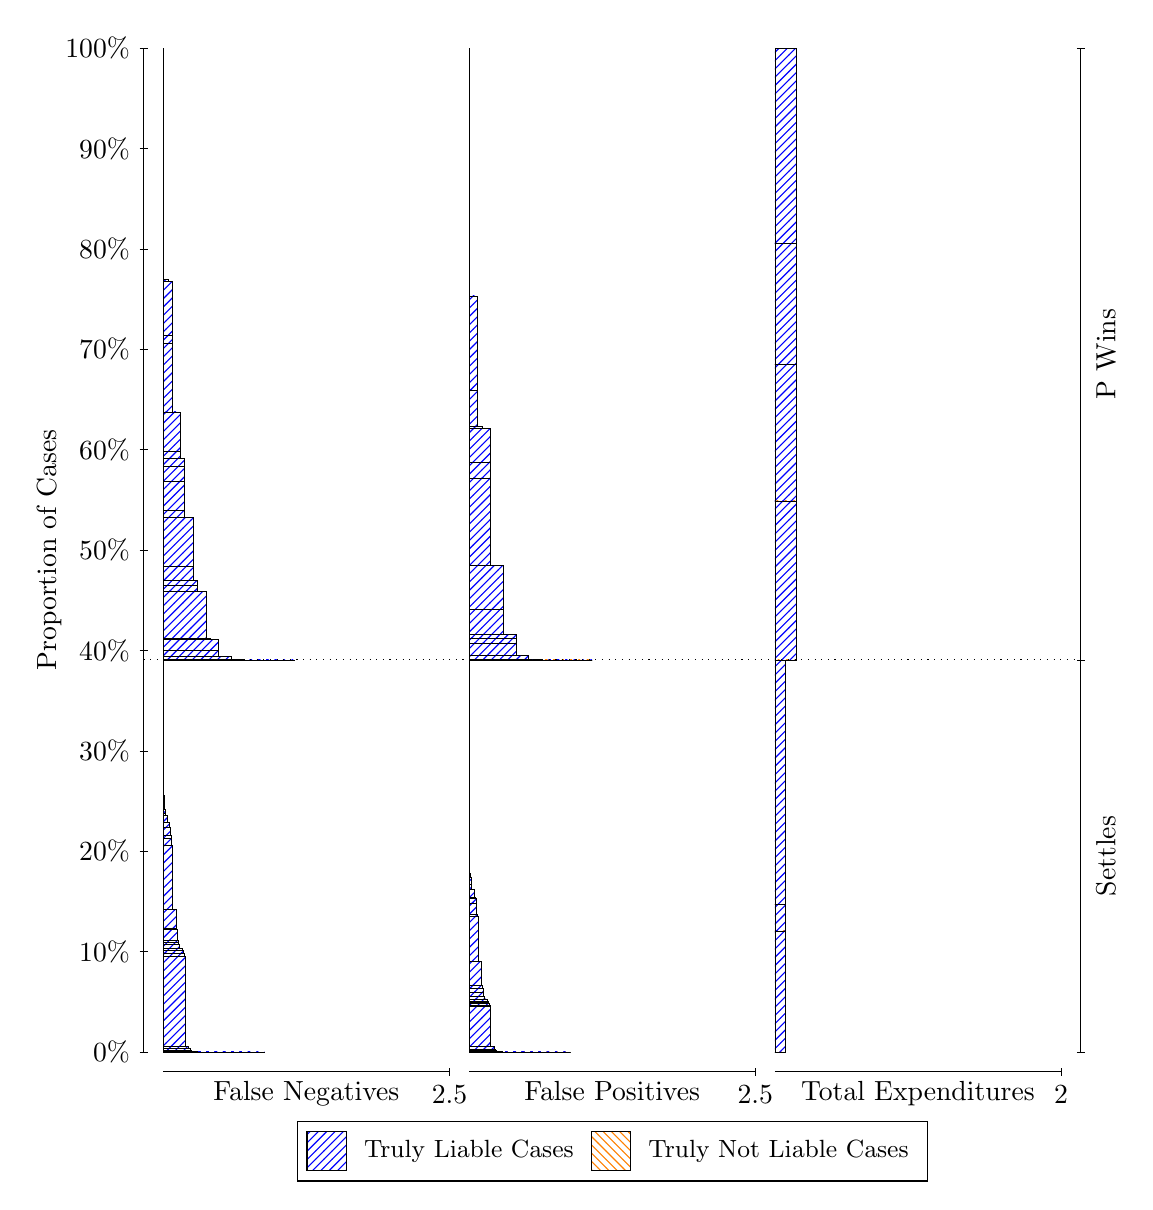
\begin{tikzpicture}
\draw[black, very thin] (1.5,1.75) -- (1.5,14.5);
\node[rotate=90, text=black, anchor=center] at (0.3, 8.125) {Proportion of Cases};
\draw[black, very thin] (1.45,1.75) -- (1.55,1.75);
\node[text=black, anchor=east] at (1.45, 1.75) {0\%};
\draw[black, very thin] (1.45,3.025) -- (1.55,3.025);
\node[text=black, anchor=east] at (1.45, 3.025) {10\%};
\draw[black, very thin] (1.45,4.3) -- (1.55,4.3);
\node[text=black, anchor=east] at (1.45, 4.3) {20\%};
\draw[black, very thin] (1.45,5.575) -- (1.55,5.575);
\node[text=black, anchor=east] at (1.45, 5.575) {30\%};
\draw[black, very thin] (1.45,6.85) -- (1.55,6.85);
\node[text=black, anchor=east] at (1.45, 6.85) {40\%};
\draw[black, very thin] (1.45,8.125) -- (1.55,8.125);
\node[text=black, anchor=east] at (1.45, 8.125) {50\%};
\draw[black, very thin] (1.45,9.4) -- (1.55,9.4);
\node[text=black, anchor=east] at (1.45, 9.4) {60\%};
\draw[black, very thin] (1.45,10.675) -- (1.55,10.675);
\node[text=black, anchor=east] at (1.45, 10.675) {70\%};
\draw[black, very thin] (1.45,11.95) -- (1.55,11.95);
\node[text=black, anchor=east] at (1.45, 11.95) {80\%};
\draw[black, very thin] (1.45,13.225) -- (1.55,13.225);
\node[text=black, anchor=east] at (1.45, 13.225) {90\%};
\draw[black, very thin] (1.45,14.5) -- (1.55,14.5);
\node[text=black, anchor=east] at (1.45, 14.5) {100\%};

\draw[black, very thin] (13.4,1.75) -- (13.4,14.5);
\draw[black, very thin] (13.35,1.75) -- (13.45,1.75);
\node[anchor=west] at (13.35, 1.75) {};
\draw[black, very thin] (13.35,6.7292) -- (13.45,6.7292);
\node[anchor=west] at (13.35, 6.7292) {};
\draw[black, very thin] (13.35,14.5) -- (13.45,14.5);
\node[anchor=west] at (13.35, 14.5) {};

\draw[black, very thin, pattern color=blue, pattern=north east lines] (1.75,1.75) rectangle (3.0398,1.75);
\draw[black, very thin, pattern color=blue, pattern=north east lines] (1.75,1.75) rectangle (2.9672,1.75);
\draw[black, very thin, pattern color=blue, pattern=north east lines] (1.75,1.75) rectangle (2.8945,1.75);
\draw[black, very thin, pattern color=blue, pattern=north east lines] (1.75,1.75) rectangle (2.8784,1.75);
\draw[black, very thin, pattern color=blue, pattern=north east lines] (1.75,1.75) rectangle (2.8218,1.75);
\draw[black, very thin, pattern color=blue, pattern=north east lines] (1.75,1.75) rectangle (2.8057,1.75);
\draw[black, very thin, pattern color=blue, pattern=north east lines] (1.75,1.75) rectangle (2.7492,1.75);
\draw[black, very thin, pattern color=blue, pattern=north east lines] (1.75,1.75) rectangle (2.733,1.75);
\draw[black, very thin, pattern color=blue, pattern=north east lines] (1.75,1.75) rectangle (2.7169,1.75);
\draw[black, very thin, pattern color=blue, pattern=north east lines] (1.75,1.75) rectangle (2.6765,1.75);
\draw[black, very thin, pattern color=blue, pattern=north east lines] (1.75,1.75) rectangle (2.6604,1.75);
\draw[black, very thin, pattern color=blue, pattern=north east lines] (1.75,1.75) rectangle (2.6442,1.75);
\draw[black, very thin, pattern color=blue, pattern=north east lines] (1.75,1.75) rectangle (2.6038,1.75);
\draw[black, very thin, pattern color=blue, pattern=north east lines] (1.75,1.75) rectangle (2.5877,1.75);
\draw[black, very thin, pattern color=blue, pattern=north east lines] (1.75,1.75) rectangle (2.5715,1.75);
\draw[black, very thin, pattern color=blue, pattern=north east lines] (1.75,1.75) rectangle (2.5554,1.75);
\draw[black, very thin, pattern color=blue, pattern=north east lines] (1.75,1.75) rectangle (2.5312,1.75);
\draw[black, very thin, pattern color=blue, pattern=north east lines] (1.75,1.75) rectangle (2.515,1.75);
\draw[black, very thin, pattern color=blue, pattern=north east lines] (1.75,1.75) rectangle (2.4989,1.75);
\draw[black, very thin, pattern color=blue, pattern=north east lines] (1.75,1.75) rectangle (2.4827,1.75);
\draw[black, very thin, pattern color=blue, pattern=north east lines] (1.75,1.75) rectangle (2.4585,1.75);
\draw[black, very thin, pattern color=blue, pattern=north east lines] (1.75,1.75) rectangle (2.4424,1.75);
\draw[black, very thin, pattern color=blue, pattern=north east lines] (1.75,1.75) rectangle (2.4262,1.75);
\draw[black, very thin, pattern color=blue, pattern=north east lines] (1.75,1.75) rectangle (2.4101,1.75);
\draw[black, very thin, pattern color=blue, pattern=north east lines] (1.75,1.75) rectangle (2.3939,1.75);
\draw[black, very thin, pattern color=blue, pattern=north east lines] (1.75,1.75) rectangle (2.3858,1.75);
\draw[black, very thin, pattern color=blue, pattern=north east lines] (1.75,1.75) rectangle (2.3697,1.75);
\draw[black, very thin, pattern color=blue, pattern=north east lines] (1.75,1.75) rectangle (2.3535,1.75);
\draw[black, very thin, pattern color=blue, pattern=north east lines] (1.75,1.75) rectangle (2.3374,1.75);
\draw[black, very thin, pattern color=blue, pattern=north east lines] (1.75,1.75) rectangle (2.3212,1.75);
\draw[black, very thin, pattern color=blue, pattern=north east lines] (1.75,1.75) rectangle (2.3132,1.7501);
\draw[black, very thin, pattern color=blue, pattern=north east lines] (1.75,1.7501) rectangle (2.297,1.7501);
\draw[black, very thin, pattern color=blue, pattern=north east lines] (1.75,1.7501) rectangle (2.2809,1.7502);
\draw[black, very thin, pattern color=blue, pattern=north east lines] (1.75,1.7502) rectangle (2.2647,1.7503);
\draw[black, very thin, pattern color=blue, pattern=north east lines] (1.75,1.7503) rectangle (2.2486,1.7509);
\draw[black, very thin, pattern color=blue, pattern=north east lines] (1.75,1.7509) rectangle (2.2405,1.7509);
\draw[black, very thin, pattern color=blue, pattern=north east lines] (1.75,1.7509) rectangle (2.2324,1.7514);
\draw[black, very thin, pattern color=blue, pattern=north east lines] (1.75,1.7514) rectangle (2.2244,1.7514);
\draw[black, very thin, pattern color=blue, pattern=north east lines] (1.75,1.7514) rectangle (2.2082,1.7514);
\draw[black, very thin, pattern color=blue, pattern=north east lines] (1.75,1.7514) rectangle (2.1921,1.7514);
\draw[black, very thin, pattern color=blue, pattern=north east lines] (1.75,1.7514) rectangle (2.1759,1.7534);
\draw[black, very thin, pattern color=blue, pattern=north east lines] (1.75,1.7534) rectangle (2.1678,1.754);
\draw[black, very thin, pattern color=blue, pattern=north east lines] (1.75,1.754) rectangle (2.1598,1.7559);
\draw[black, very thin, pattern color=blue, pattern=north east lines] (1.75,1.7559) rectangle (2.1517,1.7574);
\draw[black, very thin, pattern color=blue, pattern=north east lines] (1.75,1.7574) rectangle (2.1355,1.7575);
\draw[black, very thin, pattern color=blue, pattern=north east lines] (1.75,1.7575) rectangle (2.1194,1.7623);
\draw[black, very thin, pattern color=blue, pattern=north east lines] (1.75,1.7623) rectangle (2.1032,1.7671);
\draw[black, very thin, pattern color=blue, pattern=north east lines] (1.75,1.7671) rectangle (2.0952,1.7728);
\draw[black, very thin, pattern color=blue, pattern=north east lines] (1.75,1.7728) rectangle (2.0871,1.7945);
\draw[black, very thin, pattern color=blue, pattern=north east lines] (1.75,1.7945) rectangle (2.079,1.7952);
\draw[black, very thin, pattern color=blue, pattern=north east lines] (1.75,1.7952) rectangle (2.0709,1.8209);
\draw[black, very thin, pattern color=blue, pattern=north east lines] (1.75,1.8209) rectangle (2.0629,1.8209);
\draw[black, very thin, pattern color=blue, pattern=north east lines] (1.75,1.8209) rectangle (2.0467,1.8209);
\draw[black, very thin, pattern color=blue, pattern=north east lines] (1.75,1.8209) rectangle (2.0306,1.8209);
\draw[black, very thin, pattern color=blue, pattern=north east lines] (1.75,1.8209) rectangle (2.0225,2.9667);
\draw[black, very thin, pattern color=blue, pattern=north east lines] (1.75,2.9667) rectangle (2.0144,2.9986);
\draw[black, very thin, pattern color=blue, pattern=north east lines] (1.75,2.9986) rectangle (2.0064,3.008);
\draw[black, very thin, pattern color=blue, pattern=north east lines] (1.75,3.008) rectangle (1.9983,3.0406);
\draw[black, very thin, pattern color=blue, pattern=north east lines] (1.75,3.0406) rectangle (1.9902,3.0636);
\draw[black, very thin, pattern color=blue, pattern=north east lines] (1.75,3.0636) rectangle (1.9741,3.0649);
\draw[black, very thin, pattern color=blue, pattern=north east lines] (1.75,3.0649) rectangle (1.9579,3.1135);
\draw[black, very thin, pattern color=blue, pattern=north east lines] (1.75,3.1135) rectangle (1.9418,3.1369);
\draw[black, very thin, pattern color=blue, pattern=north east lines] (1.75,3.1369) rectangle (1.9337,3.1687);
\draw[black, very thin, pattern color=blue, pattern=north east lines] (1.75,3.1687) rectangle (1.9256,3.3073);
\draw[black, very thin, pattern color=blue, pattern=north east lines] (1.75,3.3073) rectangle (1.9175,3.3173);
\draw[black, very thin, pattern color=blue, pattern=north east lines] (1.75,3.3173) rectangle (1.9095,3.5611);
\draw[black, very thin, pattern color=blue, pattern=north east lines] (1.75,3.5611) rectangle (1.9014,3.5616);
\draw[black, very thin, pattern color=blue, pattern=north east lines] (1.75,3.5616) rectangle (1.8852,3.5618);
\draw[black, very thin, pattern color=blue, pattern=north east lines] (1.75,3.5618) rectangle (1.8691,3.5618);
\draw[black, very thin, pattern color=blue, pattern=north east lines] (1.75,3.5618) rectangle (1.861,4.3778);
\draw[black, very thin, pattern color=blue, pattern=north east lines] (1.75,4.3778) rectangle (1.8529,4.4579);
\draw[black, very thin, pattern color=blue, pattern=north east lines] (1.75,4.4579) rectangle (1.8449,4.5047);
\draw[black, very thin, pattern color=blue, pattern=north east lines] (1.75,4.5047) rectangle (1.8368,4.5991);
\draw[black, very thin, pattern color=blue, pattern=north east lines] (1.75,4.5991) rectangle (1.8287,4.6646);
\draw[black, very thin, pattern color=blue, pattern=north east lines] (1.75,4.6646) rectangle (1.8126,4.6679);
\draw[black, very thin, pattern color=blue, pattern=north east lines] (1.75,4.6679) rectangle (1.7964,4.7614);
\draw[black, very thin, pattern color=blue, pattern=north east lines] (1.75,4.7614) rectangle (1.7803,4.7819);
\draw[black, very thin, pattern color=blue, pattern=north east lines] (1.75,4.7819) rectangle (1.7722,4.8362);
\draw[black, very thin, pattern color=blue, pattern=north east lines] (1.75,4.8362) rectangle (1.7641,4.9793);
\draw[black, very thin, pattern color=blue, pattern=north east lines] (1.75,4.9793) rectangle (1.7561,5.0075);
\draw[black, very thin, pattern color=orange, pattern=north west lines] (1.75,5.0075) rectangle (1.75,5.0075);
\draw[black, very thin, pattern color=blue, pattern=north east lines] (1.75,5.0075) rectangle (1.75,6.7292);
\draw[black, very thin, pattern color=blue, pattern=north east lines] (1.75,6.7292) rectangle (3.4213,6.7292);
\draw[black, very thin, pattern color=blue, pattern=north east lines] (1.75,6.7292) rectangle (3.2599,6.7292);
\draw[black, very thin, pattern color=blue, pattern=north east lines] (1.75,6.7292) rectangle (3.2599,6.7292);
\draw[black, very thin, pattern color=blue, pattern=north east lines] (1.75,6.7292) rectangle (3.1509,6.7292);
\draw[black, very thin, pattern color=blue, pattern=north east lines] (1.75,6.7292) rectangle (3.0984,6.7292);
\draw[black, very thin, pattern color=blue, pattern=north east lines] (1.75,6.7292) rectangle (3.0984,6.7292);
\draw[black, very thin, pattern color=blue, pattern=north east lines] (1.75,6.7292) rectangle (2.9894,6.7292);
\draw[black, very thin, pattern color=blue, pattern=north east lines] (1.75,6.7292) rectangle (2.9894,6.7292);
\draw[black, very thin, pattern color=blue, pattern=north east lines] (1.75,6.7292) rectangle (2.9369,6.7295);
\draw[black, very thin, pattern color=blue, pattern=north east lines] (1.75,6.7295) rectangle (2.8279,6.7295);
\draw[black, very thin, pattern color=blue, pattern=north east lines] (1.75,6.7295) rectangle (2.7754,6.7322);
\draw[black, very thin, pattern color=blue, pattern=north east lines] (1.75,6.7322) rectangle (2.7754,6.7341);
\draw[black, very thin, pattern color=blue, pattern=north east lines] (1.75,6.7341) rectangle (2.6664,6.7341);
\draw[black, very thin, pattern color=blue, pattern=north east lines] (1.75,6.7341) rectangle (2.6139,6.7754);
\draw[black, very thin, pattern color=blue, pattern=north east lines] (1.75,6.7754) rectangle (2.5049,6.7754);
\draw[black, very thin, pattern color=blue, pattern=north east lines] (1.75,6.7754) rectangle (2.5049,6.7756);
\draw[black, very thin, pattern color=blue, pattern=north east lines] (1.75,6.7756) rectangle (2.4524,6.8542);
\draw[black, very thin, pattern color=blue, pattern=north east lines] (1.75,6.8542) rectangle (2.4524,6.9874);
\draw[black, very thin, pattern color=blue, pattern=north east lines] (1.75,6.9874) rectangle (2.3434,6.988);
\draw[black, very thin, pattern color=blue, pattern=north east lines] (1.75,6.988) rectangle (2.3434,6.9937);
\draw[black, very thin, pattern color=blue, pattern=north east lines] (1.75,6.9937) rectangle (2.3434,6.9978);
\draw[black, very thin, pattern color=blue, pattern=north east lines] (1.75,6.9978) rectangle (2.291,7.5955);
\draw[black, very thin, pattern color=blue, pattern=north east lines] (1.75,7.5955) rectangle (2.182,7.6049);
\draw[black, very thin, pattern color=blue, pattern=north east lines] (1.75,7.6049) rectangle (2.182,7.6707);
\draw[black, very thin, pattern color=blue, pattern=north east lines] (1.75,7.6707) rectangle (2.182,7.7345);
\draw[black, very thin, pattern color=blue, pattern=north east lines] (1.75,7.7345) rectangle (2.1295,7.9219);
\draw[black, very thin, pattern color=blue, pattern=north east lines] (1.75,7.9219) rectangle (2.1295,8.5436);
\draw[black, very thin, pattern color=blue, pattern=north east lines] (1.75,8.5436) rectangle (2.0205,8.6261);
\draw[black, very thin, pattern color=blue, pattern=north east lines] (1.75,8.6261) rectangle (2.0205,8.9996);
\draw[black, very thin, pattern color=blue, pattern=north east lines] (1.75,8.9996) rectangle (2.0205,9.1862);
\draw[black, very thin, pattern color=blue, pattern=north east lines] (1.75,9.1862) rectangle (2.0205,9.2903);
\draw[black, very thin, pattern color=blue, pattern=north east lines] (1.75,9.2903) rectangle (1.968,9.3771);
\draw[black, very thin, pattern color=blue, pattern=north east lines] (1.75,9.3771) rectangle (1.968,9.8778);
\draw[black, very thin, pattern color=blue, pattern=north east lines] (1.75,9.8778) rectangle (1.859,10.751);
\draw[black, very thin, pattern color=blue, pattern=north east lines] (1.75,10.751) rectangle (1.859,10.854);
\draw[black, very thin, pattern color=blue, pattern=north east lines] (1.75,10.854) rectangle (1.859,11.532);
\draw[black, very thin, pattern color=blue, pattern=north east lines] (1.75,11.532) rectangle (1.8065,11.533);
\draw[black, very thin, pattern color=blue, pattern=north east lines] (1.75,11.533) rectangle (1.8065,11.539);
\draw[black, very thin, pattern color=blue, pattern=north east lines] (1.75,11.539) rectangle (1.8065,11.564);
\draw[black, very thin, pattern color=blue, pattern=north east lines] (1.75,11.564) rectangle (1.8065,11.564);
\draw[black, very thin, pattern color=orange, pattern=north west lines] (1.75,11.564) rectangle (1.75,11.564);
\draw[black, very thin, pattern color=blue, pattern=north east lines] (1.75,11.564) rectangle (1.75,14.5);
\draw[black, very thin, pattern color=orange, pattern=north west lines] (5.6333,1.75) rectangle (6.9232,1.75);
\draw[black, very thin, pattern color=blue, pattern=north east lines] (5.6333,1.75) rectangle (6.9232,1.75);
\draw[black, very thin, pattern color=orange, pattern=north west lines] (5.6333,1.75) rectangle (6.8505,1.75);
\draw[black, very thin, pattern color=blue, pattern=north east lines] (5.6333,1.75) rectangle (6.8505,1.75);
\draw[black, very thin, pattern color=orange, pattern=north west lines] (5.6333,1.75) rectangle (6.7778,1.75);
\draw[black, very thin, pattern color=blue, pattern=north east lines] (5.6333,1.75) rectangle (6.7778,1.75);
\draw[black, very thin, pattern color=blue, pattern=north east lines] (5.6333,1.75) rectangle (6.7617,1.75);
\draw[black, very thin, pattern color=orange, pattern=north west lines] (5.6333,1.75) rectangle (6.7052,1.75);
\draw[black, very thin, pattern color=blue, pattern=north east lines] (5.6333,1.75) rectangle (6.7052,1.75);
\draw[black, very thin, pattern color=blue, pattern=north east lines] (5.6333,1.75) rectangle (6.689,1.75);
\draw[black, very thin, pattern color=orange, pattern=north west lines] (5.6333,1.75) rectangle (6.6325,1.75);
\draw[black, very thin, pattern color=blue, pattern=north east lines] (5.6333,1.75) rectangle (6.6325,1.75);
\draw[black, very thin, pattern color=blue, pattern=north east lines] (5.6333,1.75) rectangle (6.6164,1.75);
\draw[black, very thin, pattern color=blue, pattern=north east lines] (5.6333,1.75) rectangle (6.6002,1.75);
\draw[black, very thin, pattern color=orange, pattern=north west lines] (5.6333,1.75) rectangle (6.5598,1.75);
\draw[black, very thin, pattern color=blue, pattern=north east lines] (5.6333,1.75) rectangle (6.5598,1.75);
\draw[black, very thin, pattern color=blue, pattern=north east lines] (5.6333,1.75) rectangle (6.5437,1.75);
\draw[black, very thin, pattern color=blue, pattern=north east lines] (5.6333,1.75) rectangle (6.5275,1.75);
\draw[black, very thin, pattern color=orange, pattern=north west lines] (5.6333,1.75) rectangle (6.4872,1.75);
\draw[black, very thin, pattern color=blue, pattern=north east lines] (5.6333,1.75) rectangle (6.4872,1.75);
\draw[black, very thin, pattern color=blue, pattern=north east lines] (5.6333,1.75) rectangle (6.471,1.75);
\draw[black, very thin, pattern color=blue, pattern=north east lines] (5.6333,1.75) rectangle (6.4549,1.75);
\draw[black, very thin, pattern color=blue, pattern=north east lines] (5.6333,1.75) rectangle (6.4387,1.75);
\draw[black, very thin, pattern color=orange, pattern=north west lines] (5.6333,1.75) rectangle (6.4145,1.75);
\draw[black, very thin, pattern color=blue, pattern=north east lines] (5.6333,1.75) rectangle (6.4145,1.75);
\draw[black, very thin, pattern color=blue, pattern=north east lines] (5.6333,1.75) rectangle (6.3984,1.75);
\draw[black, very thin, pattern color=blue, pattern=north east lines] (5.6333,1.75) rectangle (6.3822,1.75);
\draw[black, very thin, pattern color=blue, pattern=north east lines] (5.6333,1.75) rectangle (6.3661,1.75);
\draw[black, very thin, pattern color=orange, pattern=north west lines] (5.6333,1.75) rectangle (6.3418,1.75);
\draw[black, very thin, pattern color=blue, pattern=north east lines] (5.6333,1.75) rectangle (6.3418,1.75);
\draw[black, very thin, pattern color=blue, pattern=north east lines] (5.6333,1.75) rectangle (6.3257,1.75);
\draw[black, very thin, pattern color=blue, pattern=north east lines] (5.6333,1.75) rectangle (6.3095,1.75);
\draw[black, very thin, pattern color=blue, pattern=north east lines] (5.6333,1.75) rectangle (6.2934,1.75);
\draw[black, very thin, pattern color=blue, pattern=north east lines] (5.6333,1.75) rectangle (6.2772,1.75);
\draw[black, very thin, pattern color=orange, pattern=north west lines] (5.6333,1.75) rectangle (6.2692,1.75);
\draw[black, very thin, pattern color=blue, pattern=north east lines] (5.6333,1.75) rectangle (6.2692,1.75);
\draw[black, very thin, pattern color=blue, pattern=north east lines] (5.6333,1.75) rectangle (6.253,1.75);
\draw[black, very thin, pattern color=blue, pattern=north east lines] (5.6333,1.75) rectangle (6.2369,1.75);
\draw[black, very thin, pattern color=blue, pattern=north east lines] (5.6333,1.75) rectangle (6.2207,1.75);
\draw[black, very thin, pattern color=blue, pattern=north east lines] (5.6333,1.75) rectangle (6.2046,1.75);
\draw[black, very thin, pattern color=orange, pattern=north west lines] (5.6333,1.75) rectangle (6.1965,1.75);
\draw[black, very thin, pattern color=blue, pattern=north east lines] (5.6333,1.75) rectangle (6.1965,1.75);
\draw[black, very thin, pattern color=blue, pattern=north east lines] (5.6333,1.75) rectangle (6.1804,1.7501);
\draw[black, very thin, pattern color=blue, pattern=north east lines] (5.6333,1.7501) rectangle (6.1642,1.7501);
\draw[black, very thin, pattern color=blue, pattern=north east lines] (5.6333,1.7501) rectangle (6.1481,1.7501);
\draw[black, very thin, pattern color=blue, pattern=north east lines] (5.6333,1.7501) rectangle (6.1319,1.7504);
\draw[black, very thin, pattern color=orange, pattern=north west lines] (5.6333,1.7504) rectangle (6.1238,1.7504);
\draw[black, very thin, pattern color=blue, pattern=north east lines] (5.6333,1.7504) rectangle (6.1238,1.7504);
\draw[black, very thin, pattern color=blue, pattern=north east lines] (5.6333,1.7504) rectangle (6.1158,1.7518);
\draw[black, very thin, pattern color=blue, pattern=north east lines] (5.6333,1.7518) rectangle (6.1077,1.7518);
\draw[black, very thin, pattern color=blue, pattern=north east lines] (5.6333,1.7518) rectangle (6.0915,1.7518);
\draw[black, very thin, pattern color=blue, pattern=north east lines] (5.6333,1.7518) rectangle (6.0754,1.7518);
\draw[black, very thin, pattern color=blue, pattern=north east lines] (5.6333,1.7518) rectangle (6.0592,1.7533);
\draw[black, very thin, pattern color=orange, pattern=north west lines] (5.6333,1.7533) rectangle (6.0512,1.7533);
\draw[black, very thin, pattern color=blue, pattern=north east lines] (5.6333,1.7533) rectangle (6.0512,1.7546);
\draw[black, very thin, pattern color=blue, pattern=north east lines] (5.6333,1.7546) rectangle (6.0431,1.7557);
\draw[black, very thin, pattern color=blue, pattern=north east lines] (5.6333,1.7557) rectangle (6.035,1.7558);
\draw[black, very thin, pattern color=blue, pattern=north east lines] (5.6333,1.7558) rectangle (6.0189,1.7577);
\draw[black, very thin, pattern color=blue, pattern=north east lines] (5.6333,1.7577) rectangle (6.0027,1.7578);
\draw[black, very thin, pattern color=blue, pattern=north east lines] (5.6333,1.7578) rectangle (5.9866,1.7612);
\draw[black, very thin, pattern color=orange, pattern=north west lines] (5.6333,1.7612) rectangle (5.9785,1.7612);
\draw[black, very thin, pattern color=blue, pattern=north east lines] (5.6333,1.7612) rectangle (5.9785,1.7712);
\draw[black, very thin, pattern color=blue, pattern=north east lines] (5.6333,1.7712) rectangle (5.9704,1.7793);
\draw[black, very thin, pattern color=blue, pattern=north east lines] (5.6333,1.7793) rectangle (5.9624,1.7817);
\draw[black, very thin, pattern color=blue, pattern=north east lines] (5.6333,1.7817) rectangle (5.9543,1.8217);
\draw[black, very thin, pattern color=blue, pattern=north east lines] (5.6333,1.8217) rectangle (5.9462,1.8217);
\draw[black, very thin, pattern color=blue, pattern=north east lines] (5.6333,1.8217) rectangle (5.9301,1.8217);
\draw[black, very thin, pattern color=blue, pattern=north east lines] (5.6333,1.8217) rectangle (5.9139,1.8223);
\draw[black, very thin, pattern color=orange, pattern=north west lines] (5.6333,1.8223) rectangle (5.9058,1.8223);
\draw[black, very thin, pattern color=blue, pattern=north east lines] (5.6333,1.8223) rectangle (5.9058,2.3259);
\draw[black, very thin, pattern color=blue, pattern=north east lines] (5.6333,2.3259) rectangle (5.8978,2.3405);
\draw[black, very thin, pattern color=blue, pattern=north east lines] (5.6333,2.3405) rectangle (5.8897,2.3674);
\draw[black, very thin, pattern color=blue, pattern=north east lines] (5.6333,2.3674) rectangle (5.8816,2.3861);
\draw[black, very thin, pattern color=blue, pattern=north east lines] (5.6333,2.3861) rectangle (5.8735,2.3892);
\draw[black, very thin, pattern color=blue, pattern=north east lines] (5.6333,2.3892) rectangle (5.8574,2.4217);
\draw[black, very thin, pattern color=blue, pattern=north east lines] (5.6333,2.4217) rectangle (5.8412,2.423);
\draw[black, very thin, pattern color=blue, pattern=north east lines] (5.6333,2.423) rectangle (5.8251,2.4572);
\draw[black, very thin, pattern color=blue, pattern=north east lines] (5.6333,2.4572) rectangle (5.817,2.5126);
\draw[black, very thin, pattern color=blue, pattern=north east lines] (5.6333,2.5126) rectangle (5.8089,2.5588);
\draw[black, very thin, pattern color=blue, pattern=north east lines] (5.6333,2.5588) rectangle (5.8009,2.5912);
\draw[black, very thin, pattern color=blue, pattern=north east lines] (5.6333,2.5912) rectangle (5.7928,2.8988);
\draw[black, very thin, pattern color=blue, pattern=north east lines] (5.6333,2.8988) rectangle (5.7847,2.8988);
\draw[black, very thin, pattern color=blue, pattern=north east lines] (5.6333,2.8988) rectangle (5.7686,2.8989);
\draw[black, very thin, pattern color=blue, pattern=north east lines] (5.6333,2.8989) rectangle (5.7524,2.9003);
\draw[black, very thin, pattern color=blue, pattern=north east lines] (5.6333,2.9003) rectangle (5.7444,3.4716);
\draw[black, very thin, pattern color=blue, pattern=north east lines] (5.6333,3.4716) rectangle (5.7363,3.4999);
\draw[black, very thin, pattern color=blue, pattern=north east lines] (5.6333,3.4999) rectangle (5.7282,3.643);
\draw[black, very thin, pattern color=blue, pattern=north east lines] (5.6333,3.643) rectangle (5.7201,3.6972);
\draw[black, very thin, pattern color=blue, pattern=north east lines] (5.6333,3.6972) rectangle (5.7121,3.7178);
\draw[black, very thin, pattern color=blue, pattern=north east lines] (5.6333,3.7178) rectangle (5.6959,3.8113);
\draw[black, very thin, pattern color=blue, pattern=north east lines] (5.6333,3.8113) rectangle (5.6798,3.8146);
\draw[black, very thin, pattern color=blue, pattern=north east lines] (5.6333,3.8146) rectangle (5.6636,3.8801);
\draw[black, very thin, pattern color=blue, pattern=north east lines] (5.6333,3.8801) rectangle (5.6555,3.9744);
\draw[black, very thin, pattern color=blue, pattern=north east lines] (5.6333,3.9744) rectangle (5.6475,4.0212);
\draw[black, very thin, pattern color=blue, pattern=north east lines] (5.6333,4.0212) rectangle (5.6394,4.1014);
\draw[black, very thin, pattern color=blue, pattern=north east lines] (5.6333,4.1014) rectangle (5.6333,6.7292);
\draw[black, very thin, pattern color=orange, pattern=north west lines] (5.6333,6.7292) rectangle (7.1957,6.7292);
\draw[black, very thin, pattern color=blue, pattern=north east lines] (5.6333,6.7292) rectangle (7.1957,6.7292);
\draw[black, very thin, pattern color=orange, pattern=north west lines] (5.6333,6.7292) rectangle (7.0342,6.7292);
\draw[black, very thin, pattern color=blue, pattern=north east lines] (5.6333,6.7292) rectangle (7.0342,6.7292);
\draw[black, very thin, pattern color=orange, pattern=north west lines] (5.6333,6.7292) rectangle (6.8727,6.7292);
\draw[black, very thin, pattern color=blue, pattern=north east lines] (5.6333,6.7292) rectangle (6.8727,6.7292);
\draw[black, very thin, pattern color=blue, pattern=north east lines] (5.6333,6.7292) rectangle (6.8727,6.7292);
\draw[black, very thin, pattern color=blue, pattern=north east lines] (5.6333,6.7292) rectangle (6.7112,6.7294);
\draw[black, very thin, pattern color=orange, pattern=north west lines] (5.6333,6.7294) rectangle (6.7112,6.7294);
\draw[black, very thin, pattern color=blue, pattern=north east lines] (5.6333,6.7294) rectangle (6.7112,6.7296);
\draw[black, very thin, pattern color=orange, pattern=north west lines] (5.6333,6.7296) rectangle (6.6022,6.7296);
\draw[black, very thin, pattern color=blue, pattern=north east lines] (5.6333,6.7296) rectangle (6.6022,6.7296);
\draw[black, very thin, pattern color=orange, pattern=north west lines] (5.6333,6.7296) rectangle (6.5497,6.7296);
\draw[black, very thin, pattern color=blue, pattern=north east lines] (5.6333,6.7296) rectangle (6.5497,6.7355);
\draw[black, very thin, pattern color=orange, pattern=north west lines] (5.6333,6.7355) rectangle (6.4407,6.7355);
\draw[black, very thin, pattern color=blue, pattern=north east lines] (5.6333,6.7355) rectangle (6.4407,6.7355);
\draw[black, very thin, pattern color=orange, pattern=north west lines] (5.6333,6.7355) rectangle (6.3883,6.7355);
\draw[black, very thin, pattern color=blue, pattern=north east lines] (5.6333,6.7355) rectangle (6.3883,6.7858);
\draw[black, very thin, pattern color=blue, pattern=north east lines] (5.6333,6.7858) rectangle (6.2793,6.7858);
\draw[black, very thin, pattern color=orange, pattern=north west lines] (5.6333,6.7858) rectangle (6.2793,6.7858);
\draw[black, very thin, pattern color=blue, pattern=north east lines] (5.6333,6.7858) rectangle (6.2793,6.7858);
\draw[black, very thin, pattern color=orange, pattern=north west lines] (5.6333,6.7858) rectangle (6.2268,6.7858);
\draw[black, very thin, pattern color=blue, pattern=north east lines] (5.6333,6.7858) rectangle (6.2268,6.9444);
\draw[black, very thin, pattern color=blue, pattern=north east lines] (5.6333,6.9444) rectangle (6.2268,7.0085);
\draw[black, very thin, pattern color=blue, pattern=north east lines] (5.6333,7.0085) rectangle (6.2268,7.0525);
\draw[black, very thin, pattern color=blue, pattern=north east lines] (5.6333,7.0525) rectangle (6.1178,7.0525);
\draw[black, very thin, pattern color=orange, pattern=north west lines] (5.6333,7.0525) rectangle (6.1178,7.0525);
\draw[black, very thin, pattern color=blue, pattern=north east lines] (5.6333,7.0525) rectangle (6.1178,7.0525);
\draw[black, very thin, pattern color=orange, pattern=north west lines] (5.6333,7.0525) rectangle (6.0653,7.0525);
\draw[black, very thin, pattern color=blue, pattern=north east lines] (5.6333,7.0525) rectangle (6.0653,7.3733);
\draw[black, very thin, pattern color=blue, pattern=north east lines] (5.6333,7.3733) rectangle (6.0653,7.9278);
\draw[black, very thin, pattern color=blue, pattern=north east lines] (5.6333,7.9278) rectangle (5.9563,7.9278);
\draw[black, very thin, pattern color=orange, pattern=north west lines] (5.6333,7.9278) rectangle (5.9563,7.9278);
\draw[black, very thin, pattern color=blue, pattern=north east lines] (5.6333,7.9278) rectangle (5.9563,7.928);
\draw[black, very thin, pattern color=orange, pattern=north west lines] (5.6333,7.928) rectangle (5.9038,7.928);
\draw[black, very thin, pattern color=blue, pattern=north east lines] (5.6333,7.928) rectangle (5.9038,9.0422);
\draw[black, very thin, pattern color=blue, pattern=north east lines] (5.6333,9.0422) rectangle (5.9038,9.2378);
\draw[black, very thin, pattern color=blue, pattern=north east lines] (5.6333,9.2378) rectangle (5.9038,9.6651);
\draw[black, very thin, pattern color=blue, pattern=north east lines] (5.6333,9.6651) rectangle (5.7948,9.6652);
\draw[black, very thin, pattern color=orange, pattern=north west lines] (5.6333,9.6652) rectangle (5.7948,9.6652);
\draw[black, very thin, pattern color=blue, pattern=north east lines] (5.6333,9.6652) rectangle (5.7948,9.6959);
\draw[black, very thin, pattern color=blue, pattern=north east lines] (5.6333,9.6959) rectangle (5.7948,9.6968);
\draw[black, very thin, pattern color=blue, pattern=north east lines] (5.6333,9.6968) rectangle (5.7423,10.159);
\draw[black, very thin, pattern color=blue, pattern=north east lines] (5.6333,10.159) rectangle (5.7423,11.351);
\draw[black, very thin, pattern color=orange, pattern=north west lines] (5.6333,11.351) rectangle (5.6333,11.351);
\draw[black, very thin, pattern color=blue, pattern=north east lines] (5.6333,11.351) rectangle (5.6333,14.5);
\draw[black, very thin, pattern color=orange, pattern=north west lines] (9.5167,1.75) rectangle (9.6529,1.75);
\draw[black, very thin, pattern color=blue, pattern=north east lines] (9.5167,1.75) rectangle (9.6529,3.2891);
\draw[black, very thin, pattern color=orange, pattern=north west lines] (9.5167,3.2891) rectangle (9.6529,3.2891);
\draw[black, very thin, pattern color=blue, pattern=north east lines] (9.5167,3.2891) rectangle (9.6529,3.6213);
\draw[black, very thin, pattern color=orange, pattern=north west lines] (9.5167,3.6213) rectangle (9.6529,3.6213);
\draw[black, very thin, pattern color=blue, pattern=north east lines] (9.5167,3.6213) rectangle (9.6529,6.7292);
\draw[black, very thin, pattern color=orange, pattern=north west lines] (9.5167,6.7292) rectangle (9.7892,6.7292);
\draw[black, very thin, pattern color=blue, pattern=north east lines] (9.5167,6.7292) rectangle (9.7892,8.7494);
\draw[black, very thin, pattern color=orange, pattern=north west lines] (9.5167,8.7494) rectangle (9.7892,8.7494);
\draw[black, very thin, pattern color=blue, pattern=north east lines] (9.5167,8.7494) rectangle (9.7892,10.482);
\draw[black, very thin, pattern color=orange, pattern=north west lines] (9.5167,10.482) rectangle (9.7892,10.482);
\draw[black, very thin, pattern color=blue, pattern=north east lines] (9.5167,10.482) rectangle (9.7892,12.021);
\draw[black, very thin, pattern color=orange, pattern=north west lines] (9.5167,12.021) rectangle (9.7892,12.021);
\draw[black, very thin, pattern color=blue, pattern=north east lines] (9.5167,12.021) rectangle (9.7892,14.5);
\draw[black, dotted] (1.5,6.7292) -- (13.4,6.7292);
\draw[black, very thin] (1.75,1.5) -- (5.3833,1.5);
\node[text=black, anchor=north] at (3.5667, 1.5) {False Negatives};
\draw[black, very thin] (5.3833,1.45) -- (5.3833,1.55);
\node[text=black, anchor=north] at (5.3833, 1.45) {2.5};

\draw[black, very thin] (5.6333,1.5) -- (9.2667,1.5);
\node[text=black, anchor=north] at (7.45, 1.5) {False Positives};
\draw[black, very thin] (9.2667,1.45) -- (9.2667,1.55);
\node[text=black, anchor=north] at (9.2667, 1.45) {2.5};

\draw[black, very thin] (9.5167,1.5) -- (13.15,1.5);
\node[text=black, anchor=north] at (11.333, 1.5) {Total Expenditures};
\draw[black, very thin] (13.15,1.45) -- (13.15,1.55);
\node[text=black, anchor=north] at (13.15, 1.45) {2};

\node[text=black, centered, rotate=90] at (13.72, 4.2396) {Settles};
\node[text=black, centered, rotate=90] at (13.72, 10.615) {P Wins};

\draw (7.449999999999999,1.5) node[draw=none] (baseCoordinate) {};
\begin{scope}[align=center]
        \matrix[scale=0.5, draw=black, below=0.5cm of baseCoordinate, nodes={draw}, column sep=0.1cm]{
            \node[rectangle, draw, minimum width=0.5cm, minimum height=0.5cm, pattern color=blue, pattern=north east lines] {}; &
            \node[draw=none, font=\small, text=black] (B) {Truly Liable Cases}; &
            \node[rectangle, draw, minimum width=0.5cm, minimum height=0.5cm, pattern color=orange, pattern=north west lines] {}; &
            \node[draw=none, font=\small, text=black] (B) {Truly Not Liable Cases}; \\
            };
\end{scope}

\end{tikzpicture}
\end{document}